\documentclass[11pt]{article}
\usepackage{placeins}
\usepackage{graphicx}
\usepackage{url}

\begin{document}

\begin{titlepage}
	\begin{center}
    	
\includegraphics[scale=0.10]{du.png}\par
		\begin{Huge}
			\textsc{University of Dhaka}\par
		\end{Huge}
		\begin{Large}
			Department of Computer Science and Engineering\par \vspace{.5cm}
			CSE-3111 : Computer Networking Lab \\[12pt]	
			Lab Report 7:Implementation of Link State Algorithm
		\end{Large}
	\end{center}  	
	\begin{large}
		\textbf{Submitted By:\\[12pt]}
			Name : Tasfia Tabassum\\[8pt]
			Roll No : 24\\[12pt]
			Name : Saima Akter\\[8pt]
			Roll No : 30\\[12pt]
		\textbf{Submitted On : \\[12pt]}
			March 23, 2023\\[20pt]
		\textbf{Submitted To :\\[12pt]}
			Dr. Md. Abdur Razzaque\\[12pt]
                Md Mahmudur Rahman\\[12pt]
                Md. Ashraful Islam\\[12pt]
                Md. Fahim Arefin
	\end{large}
\end{titlepage}

\section{Introduction}
The link state algorithm is a routing protocol that is used to determine the shortest path between two points in a computer network. It is a dynamic routing algorithm that uses information about the network topology to calculate the best path for data to travel. In the link state algorithm, each router maintains a database of the network's topology and updates it whenever there is a change in the network. This information is then shared with other routers in the network, allowing each router to calculate the shortest path to a destination. The link state algorithm is used in many computer networks, including the Internet, and is known for its efficiency and accuracy in finding the best routes.

\subsection{Objectives}
\begin{itemize}
    \item Our objective is to understand and implement the Link State Algorithm ,the network
topology used, and the methods employed for simulating the LSP distribution and topology updates.

\end{itemize}
%%%%
%%%%
\section{Theory}
The Link State Algorithm is a routing protocol used in computer networks to calculate the shortest path between two nodes. This algorithm is based on the concept of creating a detailed map of the network topology, including information about the state and cost of each link.

In a network using the Link State Algorithm, each node maintains a database of information about the network. This information includes the state of each link, such as whether it is up or down, and the cost of using that link. Nodes exchange information with their neighboring nodes to build a complete picture of the network topology.

Once all nodes have gathered information about the network, they use a shortest path algorithm, such as Dijkstra's algorithm, to calculate the shortest path to every other node in the network. The resulting shortest path tree is used to determine the best path to forward packets.

One of the main advantages of the Link State Algorithm is that it is highly scalable and can be used in large networks with many nodes. Additionally, it is very robust and can quickly adapt to changes in the network topology. However, the Link State Algorithm requires more processing power and memory than other routing protocols, and it can be more difficult to configure and manage.


\section{Methodology}

\subsection{Router}

In the context of the Link State Algorithm, a router is a network device that forwards packets between different networks. The router uses information about the network topology, which is provided by the server and stored in its own Link State Database (LSDB), to determine the best path for each packet.

When a router receives a packet, it looks up the destination address in its routing table and forwards the packet along the appropriate path. The router uses a shortest path algorithm, such as Dijkstra's algorithm, to calculate the shortest path to the destination based on the information in its LSDB.

If the network topology changes, such as a link going down or a new node joining the network, the router receives updated LSAs from the server and updates its own LSDB accordingly. The router then recalculates the shortest path to each destination and updates its routing table accordingly.


\subsection{Broadcaster}

In the context of the Link State Algorithm, a broadcaster refers to a network node that is responsible for broadcasting Link State Advertisements (LSAs) to other nodes in the network. The broadcaster is often the server or a router, but any node in the network can act as a broadcaster.

The broadcaster's main role is to periodically broadcast LSAs to all nodes in the network, which contain information about the state and cost of each link in the network, as well as the identity of other nodes in the network. This information is used by other nodes in the network to build a database of the network topology and calculate the shortest path to other nodes.

If the broadcaster detects a change in the network topology, such as a link going down or a new node joining the network, it sends out its own LSA to notify other nodes of the change. This ensures that all nodes in the network have up-to-date information about the network topology and can make informed routing decisions.


\subsection{Receiver}

In the context of the Link State Algorithm, a receiver refers to a network node that receives Link State Advertisements (LSAs) from a broadcaster, such as a server or router. The receiver uses this information to build a database of the network topology and calculate the shortest path to other nodes in the network.

When a receiver receives an LSA from a broadcaster, it updates its own database of the network topology and recalculates the shortest path to each node in the network. If a receiver detects a change in the network topology, such as a link going down or a new node joining the network, it updates its own database and recalculates the shortest path to each node accordingly.

The receiver's main role is to use the information provided by the broadcaster to make informed routing decisions. By building a database of the network topology and calculating the shortest path to other nodes, the receiver can forward packets along the most efficient path to their destination.



\subsection{Algorithm to implement link state algorithm : }
The graph we implemented using link state algorithm is given below:
 \begin{figure}[!h]
\centering
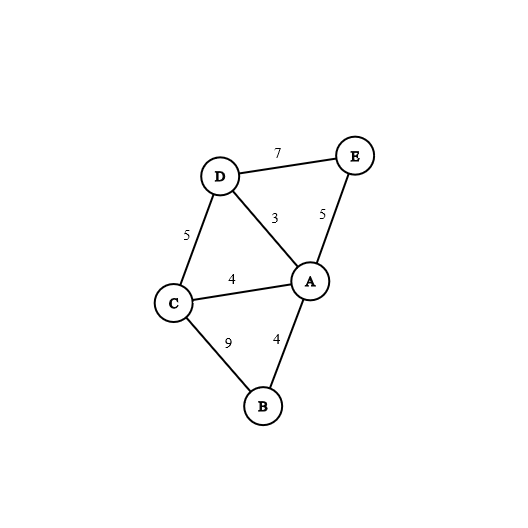
\includegraphics[width=\textwidth,height=10cm,keepaspectratio]{graph.png}
\caption{Graph Model of Routers}
\end{figure}
\FloatBarrier

\textbf{Table of each Node within cost}\\[24pt]

Table for 'A' from the graph:\\[12pt] 
\begin{tabular}{ | m{8em} | m{5cm}| } 
  \hline
   A & 0\\ 
  \hline
  B & 4\\ 
  \hline
  D & 3\\ 
  \hline
\end{tabular}\\[24pt]


Table for 'B' from the graph:\\[12pt] 
\begin{tabular}{ | m{8em} | m{5cm}| } 
  \hline
   B & 0\\ 
  \hline
  C & 9\\ 
  \hline
\end{tabular}\\[24pt]


Table for 'C' from the graph:\\[12pt] 
\begin{tabular}{ | m{8em} | m{5cm}| } 
  \hline
   C & 0\\ 
  \hline
  D & 5\\ 
  \hline
  A & 4\\ 
  \hline
\end{tabular}\\[24pt]


Table for 'D' from the graph:\\[12pt] 
\begin{tabular}{ | m{8em} | m{5cm}| } 
  \hline
   D & 0\\ 
  \hline
  E & 7\\ 
  \hline
\end{tabular}\\[24pt]


Table for 'E' from the graph:\\[12pt] 
\begin{tabular}{ | m{8em} | m{5cm}| } 
  \hline
   E & 0\\ 
  \hline
  A & 5\\ 
  \hline
\end{tabular}\\[24pt]

\textbf{Step 1: }\\[12pt]
The first step is an initialization step. Each node in the network initializes its own routing table with information about its own state (e.g., its own IP address), and sets the cost to reach all other nodes in the network to infinity.


\textbf{Step 2: }\\[12pt]
The next step is to create Link State Advertisement. Each node creates a packet called a Link State Advertisement (LSA) that contains information about its own state and the state of its directly connected neighbors. This information includes the node's ID, its neighbors' IDs, and the cost of each link to its neighbors.

\textbf{Step 3: }\\[12pt]
The next step is to create LSA flooding. Each node floods its LSA to all other nodes in the network. When a node receives an LSA, it stores the information in its own database and forwards the LSA to all of its neighbors (except the neighbor it received it from).\\[12pt]
\textbf{Method to create LSA flooding }\\[12pt]
\begin{verbatim}
def message_to_neighbour(msg):
	for nei in neighbour:
		n_ip=''
		n_port=ipport[nei]
		cl=socket.socket()
		try:
			cl.connect((n_ip,n_port))
			cl.send(msg.encode())
		except:
			print(f"{curr} unable to connect with neigbour {nei} on port the {n_port}")
		cl.close()
def message_parse(msg):
	tmp=msg
	msg=msg.split('\n')
	id,ttl=msg[0].split()
	if id==curr:
		return
	else:
		message_to_neighbour(tmp)
		dat=msg[1].split('@')
		for line in dat:
			try:
				src,dest,weight=line.split()
			except:
				break
			if src not in G:
				G[src]={}
			if dest not in G:
				G[dest]={}
			G[src][dest]=weight
			G[dest][src]=weight
		print('\nG updated\n')
		#print(G)
		parentsmap,nodecost=dijkstra(G,curr)
		print_cost(nodecost,parentsmap
\end{verbatim}
\\[12pt]

    1. The $message_to_neighbour(msg)$ function takes a message msg as input and sends it to all the neighbors of the current node (curr).\\

    2.  For each neighbor nei, the function retrieves the IP address and port number from a dictionary ipport using the neighbor's name as key.\\

    3. The function then creates a socket and attempts to connect to the neighbor using the retrieved IP address and port number.\\

    4.  If the connection is successful, the function sends the message as a byte string using the socket's send() method. Otherwise, it prints an error message indicating that the connection could not be established.\\

    Finally, the function closes the socket.\\

    5. The $message_parse(msg)$ function takes a message msg as input and parses it to extract the source node, destination node, and weight of each edge in the message.\\

    6. The message is split into two parts: the first part contains an ID and TTL, and the second part contains a series of lines separated by a delimiter ('@').\\

    7. If the ID in the message matches the current node (curr), then the function returns without doing anything, since the message has already been processed.\\

    8. Otherwise, the function sends the original message to all neighbors of the current node using the $message_to_neighbour()$ function.\\

    9. The function then loops over the lines in the message, and for each line, it extracts the source node, destination node, and weight using the $split()$ method.\\

    10. If either the source node or destination node is not already in the graph G, then the function adds them as new nodes to the graph.\\

    11. The function then adds the edge to the graph, with the weight as the edge weight. Since the graph is undirected, it adds the edge in both directions.\\

    12. The function prints a message indicating that the graph has been updated, and then runs Dijkstra's algorithm on the updated graph to compute the shortest paths and costs from the current node to all other nodes.\\

    13. Finally, the function calls the $print_cost()$ function to print the costs and paths for each node in the graph.\\



\textbf{Step 4: }\\[12pt]
The next step is to calculate shortest path. Once each node has received LSAs from all other nodes in the network, it can calculate the shortest path to each destination node using Dijkstra's algorithm. Dijkstra's algorithm calculates the shortest path by repeatedly selecting the node with the lowest cost and updating the cost of its neighbors accordingly.

\textbf{Step 5: }\\[12pt]
The next step is to calculate routing table. Each node uses the results of the shortest path calculation to update its routing table. The routing table specifies the next hop for each destination node and the total cost of reaching that node.

\textbf{Step 6: }\\[12pt]
The next step is to update LSA. Each node periodically sends updated LSAs to all other nodes in the network. These updates are triggered by changes in the node's own state or the state of its neighbors. When a node receives an updated LSA, it repeats the shortest path calculation and routing table calculation steps.\\[12pt]
\textbf{Method Used to Update LSA }\\[12pt] 
\begin{verbatim}

def graph_update():
	while True:
		time.sleep(20)
		id=curr+' 60\n'
		s=''
		node=chr(random.randrange(65, 65 + 4))
		cost=random.randint(1,50)
		if node==curr:
			continue
		G[curr][node]=cost
		G[node][curr]=cost
		print(f"Updating cost in the graph {curr} {node} {cost}")
		s+=curr+' '+str(node)+' '+str(cost)+'@'
		if s!='':
			msg=id+s
			message_to_neighbour(msg)
			parentsmap,nodecost=dijkstra(G,curr)
			print_cost(nodecost,parentsmap)
\end{verbatim}
\\
    1. The $graph update()$ function runs an infinite loop, and sleeps for 20 seconds in each iteration.\\

    2. In each iteration, the function generates a random node (letter 'A', 'B', 'C', or 'D') and a random cost between 1 and 50.\\

    3. If the randomly generated node is the same as the current node (curr), then the function continues to the next iteration of the loop without making any changes to the graph.\\

    4. If the randomly generated node is different from the current node, then the function updates the cost of the edge between the current node and the randomly generated node in the graph G.\\

    5. The function then prints a message to the console indicating the update, in the form of "Updating cost in the graph [current node] [random node] [random cost]".\\

    6. The function constructs a message msg consisting of the current node, the randomly generated node, and the random cost, separated by spaces and followed by a delimiter ('@').\\

    7. The function sends this message to its neighbors using the
 $message to neighbour()$ function.\\

    8. The function then runs Dijkstra's algorithm on the updated graph G using the dijkstra() function. This function returns two values: a dictionary parentsmap mapping each node to its parent in the shortest path tree, and a dictionary nodecost mapping each node to its cost in the shortest path tree.\\

    9. The function then calls the $print cost()$ function, which prints the cost of the shortest path from the current node to each node in the graph, as well as the path itself.\\

    
This process repeats periodically to ensure that all nodes have up-to-date information about the network topology.

\subsection{Screenshots output demonstrating the correct functionality of the program in various network scenarios: }
\textbf{Screenshots of router 1 : }\\[12pt]
 \begin{figure}[!h]
\centering
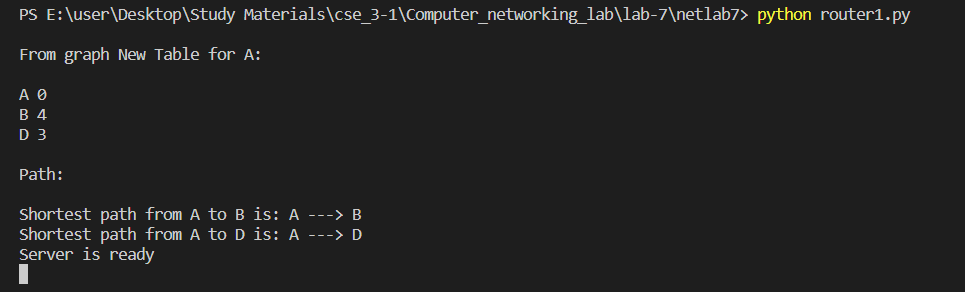
\includegraphics[width=\textwidth]{r1.png}
\caption{snapshot of Router 1}
\end{figure}
\FloatBarrier

\textbf{Screenshots of router 2 : }\\[12pt]
 \begin{figure}[!h]
\centering
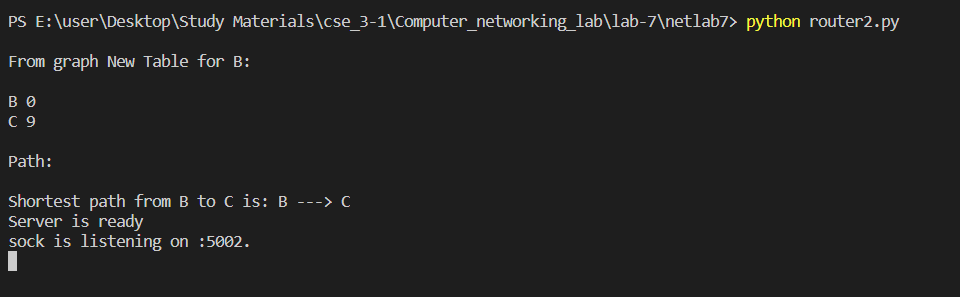
\includegraphics[width=\textwidth]{r2.png}
\caption{Snapshot of Router 2}
\end{figure}
\FloatBarrier

\textbf{Screenshots of router 3 : }\\[12pt]
 \begin{figure}[!h]
\centering
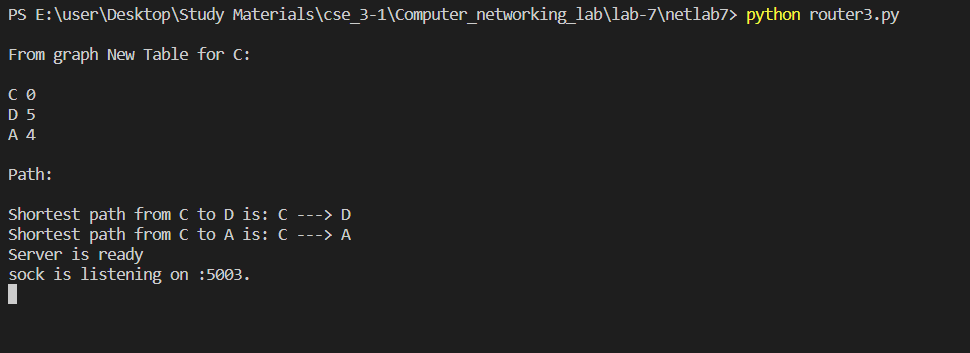
\includegraphics[width=\textwidth]{r3.png}
\caption{Snapshot of Router 3}
\end{figure}
\FloatBarrier

\textbf{Screenshots of router 4 : }\\[12pt]
 \begin{figure}[!h]
\centering
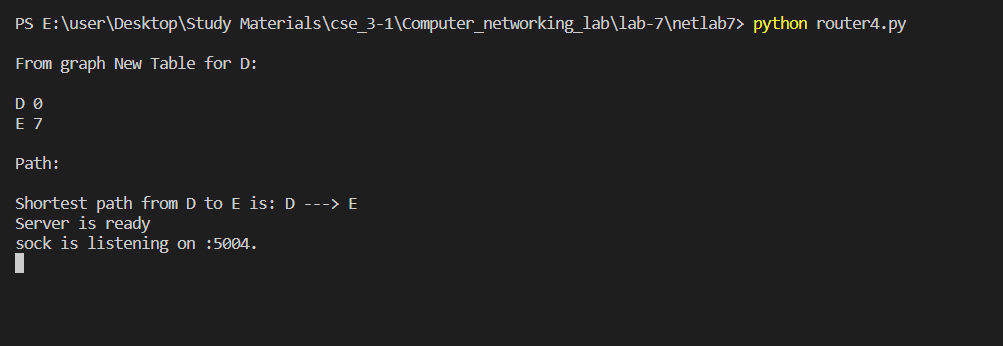
\includegraphics[width=\textwidth]{r4.png}
\caption{Snapshot of Router 4}
\end{figure}
\FloatBarrier

\textbf{Screenshots of router 5 : }\\[12pt]
 \begin{figure}[!h]
\centering
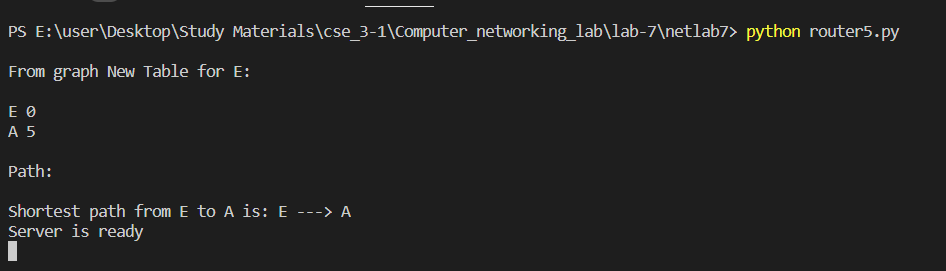
\includegraphics[width=\textwidth]{r5.png}
\caption{Snapshot of Router 5}
\end{figure}
\FloatBarrier

\subsection{Screenshots output after updating cost }
\textbf{Screenshots of router 1 after Updating cost: }\\[12pt]
 \begin{figure}[!h]
\centering
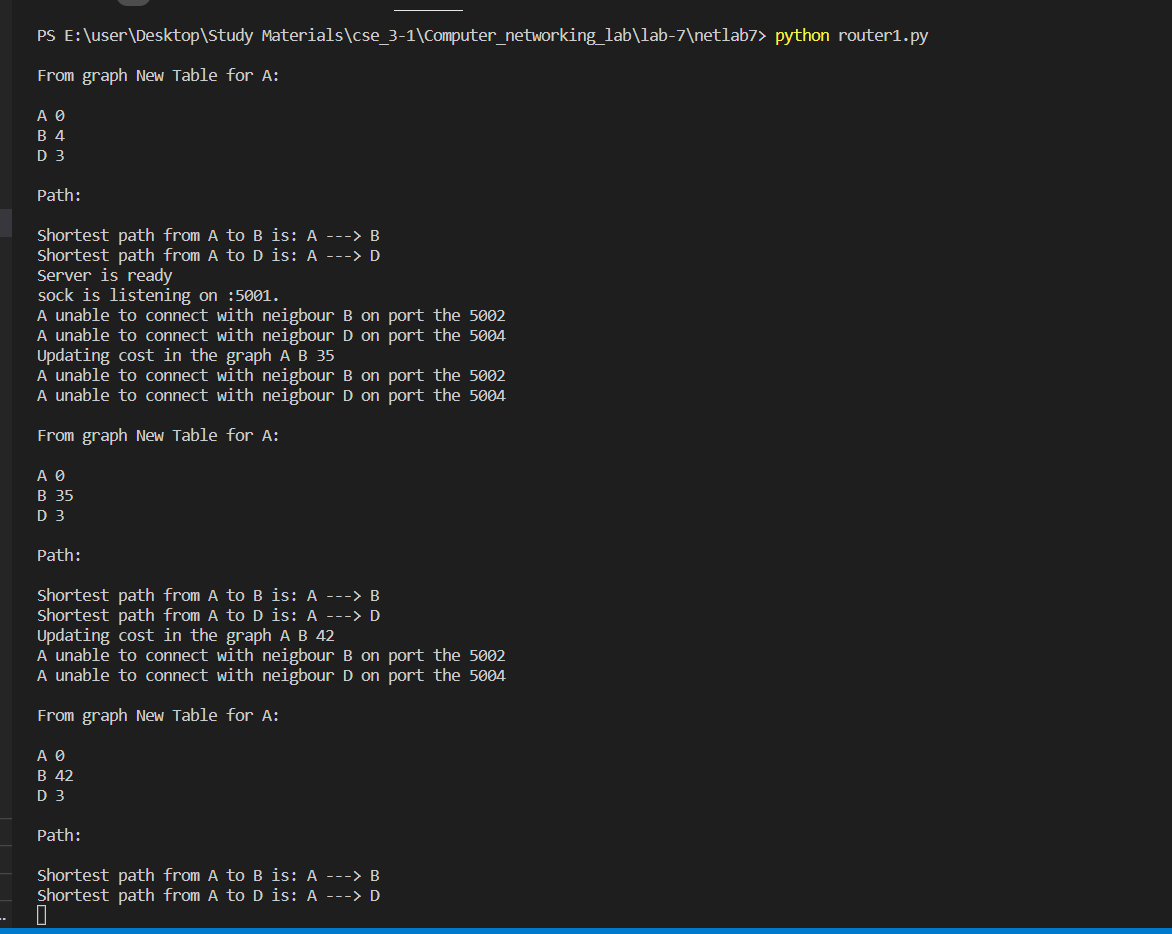
\includegraphics[width=\textwidth]{r1u.png}
\caption{snapshot of Router 1 after update}
\end{figure}
\FloatBarrier

\textbf{Screenshots of router 2 after Updating cost: }\\[12pt]
 \begin{figure}[!h]
\centering
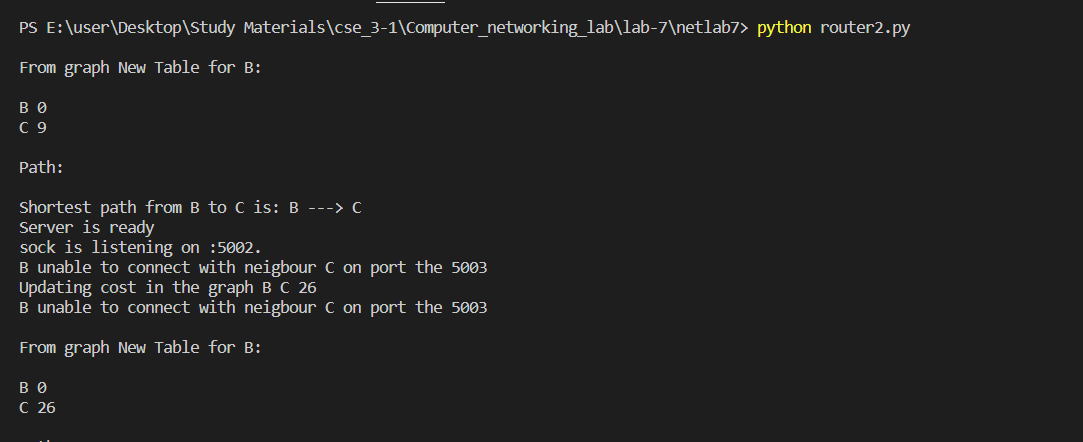
\includegraphics[width=\textwidth]{r2u.png}
\caption{snapshot of Router 2 after update}
\end{figure}
\FloatBarrier

\textbf{Screenshots of router 3 after Updating cost: }\\[12pt]
 \begin{figure}[!h]
\centering
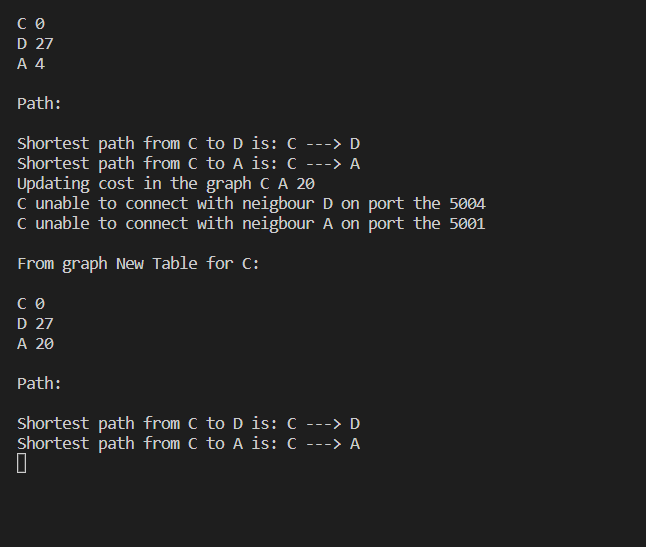
\includegraphics[width=\textwidth]{r3u.png}
\caption{snapshot of Router 3 after update}
\end{figure}
\FloatBarrier

 \subsection{Analyze Results for Link State Algorithm}
 
\textbf{Time Complexity of Link State Algorithm: }\\[12pt]
The time complexity of the link state algorithm depends on the implementation and the size ot the network. In general, it has a time complexity of $O(N^2)$, where N is the number of nodes in the network. However, this can be improved to $O(N * logN)$ using a heap data structure to implement Dijkastra's algorithm. That is why we have implemented heap in out algorithm to make it more efficient.

 \textbf{Memory Usage of Link State Algorithm: }\\[12pt]
 The memory usage of the Link State Algorithm (LSA) can vary depending on the size of the network and the number of nodes and links that need to be stored in memory.

 At a minimum, each node in the network needs to maintain a copy of the Link State Database (LSDB), which contains information about the state and cost of each link in the network. This LSDB can be quite large, especially for large networks, and can consume a significant amount of memory.

In addition to the LSDB, each node also needs to maintain information about its own state, such as its own identity and the state of its interfaces. This information typically doesn't take up as much memory as the LSDB, but it still needs to be stored somewhere.

Finally, the Link State Algorithm also requires a certain amount of memory for processing and storing messages that are exchanged between nodes in the network. This includes messages like Link State Advertisements (LSAs) and Shortest Path Tree (SPT) packets.

 \textbf{Overall analysis of performance of Link State Algorithm: }\\[12pt]
 
 The Link State Algorithm (LSA) is well-suited for large and complex networks because it calculates the shortest path to every node, allowing it to quickly adjust to changes in the network topology. This makes it a good choice for networks that require fast convergence times and high reliability. However, it can be more resource-intensive than other routing algorithms, as every node must maintain a complete view of the network topology. LSA may also face problems such as link state database synchronization issues and network partitioning, which can affect its performance. Nonetheless, LSA is widely used in many large-scale networking applications.


\section{Experience}
In the lab report on "Implementation of Link State Algorithm" we conducted a comprehensive study on the implementation of link state algorithm. While working on the experiment, we faced challenges while simulating the LSA distribution and while updating the graph. while updating the graph, to update cost, at first we tried to give update cost from user but it was not working properly so we used random function to update the cost randomly after 30 sec automatically. Another problem we faced while LSA flooding or broadcasting to neighbour, to connect to the neighbor using the retrieved IP address and port number, we first tried it with different IP address but it was not functioning, so in the end we used same IP address but different port number.



\begin{thebibliography}{1}
\bibitem{book}  Computer networking : a top-down approach 6th ed.
\bibitem{StackOverflow} StackOverflow : \url{http://stackoverflow.com/}
\bibitem{Geeks for geeks} GeeksforGeeks : \url{https://www.geeksforgeeks.org/}
\end{thebibliography}

\end{document}